\documentclass[xcolor={dvipsnames}]{beamer}
\usepackage{HECbeamer}
%  \usepackage{pgfpages}
%  \pgfpagesuselayout{4 on 1}[letterpaper,landscape, border shrink=5mm]
% \usepackage{listings}
% \usepackage{minted}
% \usemintedstyle{vs}
% \newcommand{\saskeyword}[1]{\textcolor{blue}{#1}}
% \newenvironment{sasminted}{\VerbatimEnvironment\begin{minted}[escapeinside=||,fontsize=\small,baselinestretch=1, samepage=true]{sas}}
%  {\end{minted}}

\uselanguage{French}
\languagepath{French}
\title[\color{white}{MATH60604 \S~2d Tests d'hypothèses pour modèles linéaires}]{MATH60604 \\Modélisation statistique \\ Tests d'hypothèses pour modèles linéaires}
\author{Léo Belzile}
\date{\today}
\institute{HEC Montréal\\
Département de sciences de la décision}
\date{} 

\begin{document}
\frame{\titlepage}



\section{Tests d'hypothèse}



\begin{frame}[fragile]
\frametitle{Résumé des postulats du modèle linéaire}
\be
\item \textbf{Indépendance}: les erreurs $\varepsilon_1, \ldots, \varepsilon_n$ sont des variables aléatoires \alert{indépendantes} sachant $\mathbf{X}$.
\bi
\item Cela implique que $Y_i$ est conditionellement indépendant des autres réponses sachant $\mathbf{X}_i$.
\ei
\item \textbf{Homoscédasticité}: la variance des erreurs est  \alert{constante}, soit  $\Va{\varepsilon_i}=\sigma^2$  pour $i=1, \ldots, n$. Si la variance n'est pas constante, les erreurs sont dites par opposition hétéroscédastiques.
\item \textbf{Normalité}: les erreurs, $\varepsilon$, suivent une loi \alert{normale}.
\bi \item cette supposition est uniquement requise pour la validité des tests d'hypothèse et des intervalles de confiance.
\ei
\ee
\end{frame}

\begin{frame}[fragile]
\frametitle{Résumé des postulats du modèle linéaire}
\be
\setcounter{enumi}{3}
\item \textbf{Linéarité}: la surface de réponse du modèle linéaire,
\begin{align*}
\E{Y \mid \mathrm{X}_1, \ldots, \mathrm{X}_p}=\beta_0+\beta_1\mathrm{X}_1+\ldots + \beta_p \mathrm{X}_p.
\end{align*}
est correctement spécifiée.
\bi \item L'espérance des erreurs est zéro, $\E{\varepsilon_i \mid \mathbf{X}_i}=0$ pour $i=1,\ldots, n$.
\item Toutes les variables explicatives importantes sont incluses dans le modèle.
\item Leurs effets (supposés linéaires en $\beta$) sont correctement modélisés.
\ei
\ee
\end{frame}









 \begin{frame}
\frametitle{Tests d'hypothèses pour paramètres individuels}
\bi
\item En inférence, il est souvent important de tester si l'effet d'une variable explicative est statistiquement significative. 
\item Cela revient à tester si le coefficient associé à la variable est différent de zéro,
\begin{align*}
\Hy_0: \beta_j=0,  \qquad  \Hy_1: \beta_j\neq 0                                               \end{align*}
\item Pour tester cette hypothèse bilatérale, on utilise une statistique de Wald,
\begin{align*}
t=\frac{\widehat{\beta}_j-0}{\se(\widehat{\beta}_j)}, 
\end{align*}
où $\se(\widehat{\beta}_j)$ est l'estimé de l'\textbf{erreur-type} de $\widehat{\beta}_j$. Sa distribution nulle est Student-$t$ et est rapportée par \SASlang sous le vocable \textbf{Valeur du test t}.
\ei
\end{frame}

\begin{frame}
\frametitle{Est-ce que les gens sont prêts à payer plus par carte de crédit?}
On va travailler avec l'exemple suivant inspiré de l'article
\begin{tcolorbox}[colback=lightgray!30!white,colframe=lightgray!75!black,title=Référence]
Prelec, D. et Simester, D. (2001). Always Leave Home Without It: A Further Investigation of the Credit-Card Effect on Willingness to Pay. \textit{Marketing Letters}, \textbf{12}, 5-12.
\end{tcolorbox}
\bi

\item \alert{\textbf{Question de l'étude}}: Est-ce que le fait de payer par carte de crédit encourage les gens à payer plus?
\item \textbf{Contexte}: Lors de transactions de valeurs potentiellement élevées, le montant offert par les gens devant payer par carte de crédit peut être plus élevé que celui des gens devant payer en billets.
\item \textbf{Objectifs}: Présenter de nouveaux éléments en faveur de la proposition à l'effet que les individus sont enclins à payer plus pour un produit lorsqu'ils utilisent une carte de crédit. 
\ei
\end{frame}

\begin{frame}
\frametitle{Exemple: carte de crédit vs comptant}
\bi
\item Le produit en vente: paire de billets pour le dernier match de la saison des Celtics de Boston (équipe de basketball de la NBA). Cette partie était importante, car elle allait décider qui allait terminer premier dans cette division.
\item 64 sujets répartis \textbf{au hasard} dans deux groupes:
\bi
 
\item Groupe 1 (33 sujets) : individus doivent payer comptant
\item Groupe 2 (31 sujets): individus doivent payer par carte de crédit
\ei
\item Tous les sujets ont dû remplir un questionnaire où on leur demandait combien ils étaient prêts à payer pour la paire de billets. 
\ei

\end{frame}

\begin{frame}
\frametitle{Allocation aléatoire}
\bi
\item Assigner les sujets au hasard aux différentes conditions expérimentales (groupes) s'appelle la \alert{randomisation}. 
\item \textbf{Idée}: tenter d'avoir des groupes qui sont \alert{le plus semblables possible} quant aux caractéristiques qui pourraient influencer la variable réponse et, ainsi, diminuer leur impact.
    \bi
\item il se pourrait que l'âge, le sexe, ainsi que d'autres variables, aient une influence sur le montant d'argent que la personne est prête à offrir. 
\ei
\item Autre manière de procéder: contrôler directement pour les effets de ces variables dans un modèle de  régression linéaire.
\ei
\end{frame}

\begin{frame}
\frametitle{Exemple: moyen de paiement}
La base de données \code{billets} contient des données simulées correspondant à cette étude, incluant les variables
\bi 
\item \code{offre}: montant offert (en \$) par l'individu pour se procurer les billets
\item \code{groupe}: identifie le groupe d'appartenance

\bi
 
\item  \code{groupe=0} pour les individus devant payer comptant
\item  \code{groupe=1} pour les individus devant payer avec une carte de crédit
\ei
\ei
\begin{tcolorbox}[colback=hecgrey!10!white,colframe=lightgray!75!black,title=Objectif général]
Comparer une \alert{\textbf{moyenne}} (montant moyen d'argent que les gens sont prêts à payer) entre deux groupes (carte de crédit versus comptant)
\end{tcolorbox}

\end{frame}
\begin{frame}
\frametitle{Test-$t$ pour deux échantillons avec un modèle de régression}
\bi

\item La variable \code{offre} représente le montant en dollars et la variable \code{groupe} l'indicateur binaire ($0$ pour comptant, $1$ pour crédit).
\item Le test d'égalité des moyennes est \alert{équivalent} à tester si l'effet de \code{groupe} sur l'\code{offre} est nul.
\item On peut formuler ce problème à l'aide du modèle de régression
\begin{align*}
\code{offre}= \beta_0 + \beta_1 \code{groupe} + \varepsilon
\end{align*}
\item  Tester $\Hy_0: \mu_{\code{comptant}}=\mu_{\code{crédit}}$ revient à tester $\Hy_0: \beta_1=0$.
\ei
\end{frame}

\begin{frame}[fragile]
\frametitle{Régression linéaire avec données \code{billets}}

\begin{center}
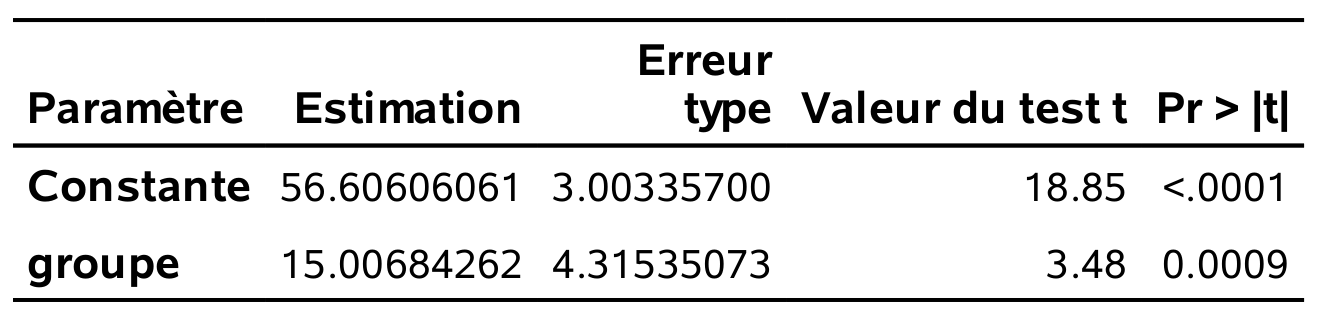
\includegraphics[width =0.9\linewidth]{img/c2/diapos3-e14}
\end{center}
\bi
\item Nous estimons que la différence \textbf{moyenne}  entre les deux groupes est $\widehat{\beta}_1=\$15$, soit des offres par crédits plus élevées. 
\item Cette différence est statistiquement significatif à niveau 5\% (valeur-$p$ de $0.0009$).
\item La sortie du modèle de régression linéaire ne contient que la valeur-$p$ du test bilatéral, mais celle du test unilatéral est moitié moindre (à cause de la symmétrie de la loi Student-$t$).
\ei
\end{frame}



 
 \begin{frame}[fragile]
\frametitle{Intervalles de confiance}
Dans \SASlang, la commande \code{clparm} ajoute les intervalles de confiance de Wald de niveau $(1-\alpha)$ (par défaut 95\%) au tableau des estimés.
\bi
\item Le code qui suit cette procédure pour le modèle régression simple
\ei
\begin{align*}
\code{intention}_i = \beta_0 + \beta_1 \code{fixation}_i + \eps_i.
\end{align*}

\begin{tcolorbox}[colback=white, colframe=hecblue, title=Code \SASlang pour ajuster le modèle linéaire]
\begin{verbatim}
proc glm data=infe.intention;
model intention=fixation / ss3 solution clparm;
run;
\end{verbatim}
\end{tcolorbox}


\end{frame}


 

\begin{frame}
\frametitle{Tests pour paramètres individuels et intervalles de confiance}

\begin{center}
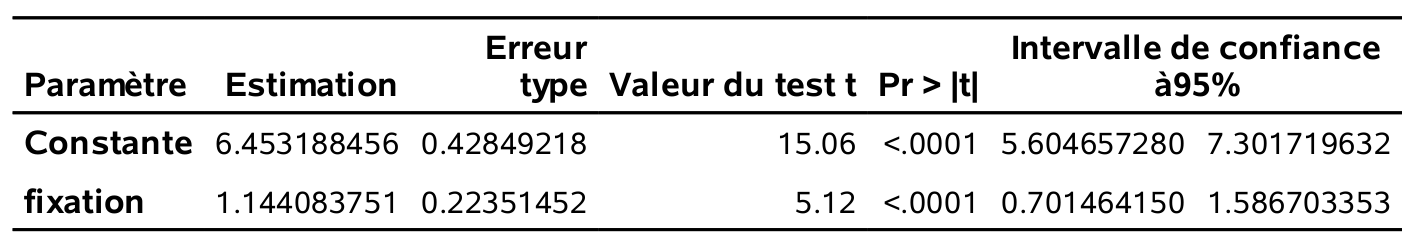
\includegraphics[width=0.9\linewidth]{img/c2/diapos3-e11}
\end{center}
\bi
\item La valeur de la statistique-$t$ pour $\Hy_0: \beta_1=0$ versus $\Hy_1:\beta_1 \neq 0$ est $t=1.144/0.224=5.12$.
\item La valeur-$p$ du test bilatéral est inférieure à $0.0001$.
\item On rejette $\Hy_0$, car il y a un effet significatif du temps de   \code{fixation} sur l'\code{intention} d'achat.
\item L'intervalle de confiance à $95$\% pour $\beta_1$, correspondant à l'effet linéaire de \code{fixation}, est $[0.70; 1.59]$. 
\item Puisque l'intervalle ne contient pas $0$, on déduit que le paramètre est significativement différent de zéro à niveau $\alpha=5$\%.
\ei
\end{frame}
% 
% \begin{frame}
% \frametitle{Simple linear regression: interpretation of the test}
% \bi
% \item It turns out that when there's one explanatory variable (simple linear regression), testing the effect of the explanatory variable on the dependent variable is equivalent to testing whether the correlation between the two variables differs from 0.
% \item We've already seen that the correlation between \code{fixation} and
% \code{intention} is significant ($p$-value $p< 0.0001$). 
% \item \alert{\textbf{Careful}: this is not true when there is more than one explanatory variable in the model}.
% % \item In this case, \code{fixation} and \code{intention} appear to be linearly related. So the model is reasonable, and testing the effect of \code{fixation} on \code{intention} is justified. Some later exemples will show that, just like in linear correlation, things are not always so simple.
% \ei
% \end{frame}

\begin{frame}[fragile]
\frametitle{Interprétation du test d'hypothèse}

Si on rejette $\Hy_0: \beta_j=0$ pour l'alternative, on exclut la possibilité qu'il n'y ait aucune \textbf{relation linéaire} significative entre $\mathrm{X}_j$ et $Y$ \textbf{une fois l'effet des autres variables pris en compte}.
% \item Même pour la régression linéaire simple, ne pas rejetter l'hypothèse nulle implique seulement qu'il n'y a pas de \textbf{relation linéaire} significative entre $\mathrm{X}_1$ et $Y$.

\begin{figure}
 \centering
 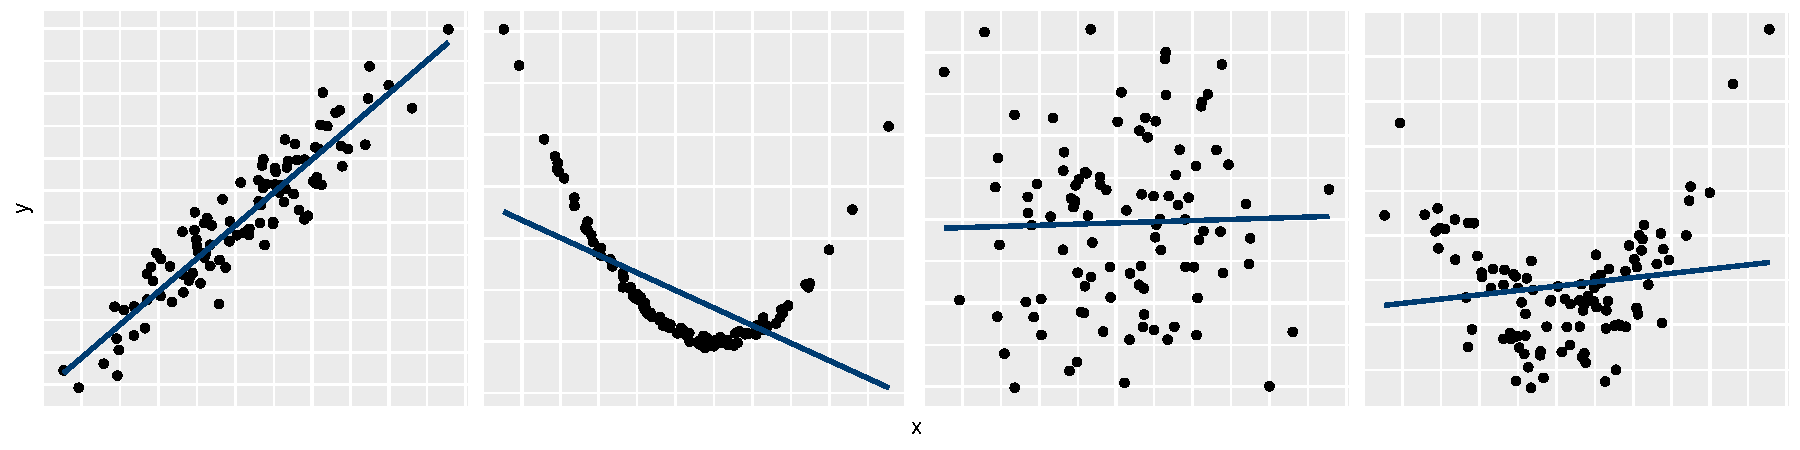
\includegraphics[width = \textwidth]{img/c2/03-linreg-fourplots}
\end{figure}
{
\footnotesize 
On rejette $\Hy_0: \beta_1 =0$ dans les deux graphiques de gauche (valeurs-$p$ moins de $10^{-6}$, mais pas dans ceux de droite (valeurs-$p$ de 0.787 et 0.156). Le coefficient de détermination est, de gauche à droite, $0.87$, $0.3$, $10^{-3}$ et $10^{-3}$.

}
\end{frame}

\begin{frame}
\frametitle{Tests d'hypothèses pour plusieurs paramètres}
\bi
\item Il est également possible de tester si \alert{plusieurs} $\beta$ sont simultanément zéros, par exemple
\begin{align*}
\Hy_0: \beta_{\code{age}}=\beta_{\code{emotion}}=0.
\end{align*}
\item Pour valider l'utilité d'une variable catégorielle, il convient également de tester pour son \alert{effet global}.
\bi 
\item La variable \code{educ} a trois niveaux et est modélisée à l'aide de deux variables indicatrices \code{educ1} et \code{educ2}; tester l'effet global d'\code{educ} revient à tester
\begin{align*}
\Hy_0: \beta_{\code{educ}_1}=\beta_{\code{educ}_2}=0.
\end{align*}
\ei
\ei
\end{frame}




\begin{frame}
\frametitle{Comparaison de modèles emboîtés}
\bi
\item Soit le  \alert{modèle complet} contenant $p$ régresseurs,
\begin{align*}
\mathbb{M}_1: Y=\beta_0+\beta_1 \mathrm{X}_1 + \cdots + \beta_g \mathrm{X}_g + \beta_{k+1}\mathrm{X}_{k+1} + \ldots + \beta_p \mathrm{X}_p + \varepsilon.
\end{align*}
\item On considère le test
\begin{align*}
\Hy_0: \beta_{k+1}=\beta_{k+2}=\ldots=\beta_p=0,
\end{align*}
\item  soit l'hypothèse que $(p-k)$ des $\beta$ (sans perte de généralité les derniers) sont simultanément zéros.
\item Le \alert{modèle contraint} contient seulement les covariables pour lesquelles $\beta_j \neq 0$,
\begin{align*}
\mathbb{M}_0: Y=\beta_0+\beta_1 \mathrm{X}_1 + \ldots + \beta_k \mathrm{X}_k + \varepsilon.
\end{align*}
\ei
\end{frame}



\begin{frame}[fragile]
\frametitle{Tests-$F$ pour comparaison de modèles imbriqués (optionnel)}
\bi
\item Soit $\mathsf{SS}_e(\mathbb{M}_1)$ la somme du carré des résidus du modèle complet $\mathbb{M}_1$,
\begin{align*}
\mathsf{SS}_e(\mathbb{M}_1)=\sum_{i=1}^n (Y_i-\hat{Y}_i^{\mathbb{M}_1})^2,
\end{align*}
où $\hat{Y}_i^{\mathbb{M}_1}$ est la  $i$e valeur ajustée du  modèle $\mathbb{M}_1$.
\item On définie de la même façon la somme du carré des résidus,  $\mathsf{SS}_e(\mathbb{M}_0)$, pour le modèle $\mathbb{M}_0$.
\item 
Logiquement, $\mathsf{SS}_e(\mathbb{M}_0) \geq \mathsf{SS}_e(\mathbb{M}_1)$ (pourquoi?)
\ei 
\end{frame}
\begin{frame}[fragile]
La statistique du test-$F$ est
\begin{align*}
F=\frac{\{\mathsf{SS}_e(\mathbb{M}_0)-\mathsf{SS}_e(\mathbb{M}_1)\}/(p-k)}{\mathsf{SS}_e(\mathbb{M}_1)/(n-p-1)}
\end{align*}
\bi 
\item Sous $\Hy_0$, la statistique-$F$  suit une  \alert{loi de Fisher} avec $(p-k)$ et $(n-p-1)$ degrés de liberté, $\mathsf{F}(p-k, n-p-1)$. 
\ei
{\footnotesize  $p-k$ est le nombre de restrictions, $n-p-1$ est la taille de l'échantillons moins le nombre de $\beta$ de $\mathbb{M}_1$.}
\end{frame}


\begin{frame}[fragile]
\frametitle{Test-$F$ pour l'effet de toutes les covariables}
\bi
\item Le premier tableau de la sortie \SASlang avec la procédure \code{glm} donne le résultat du test global pour tous les coefficients $\Hy_0: \beta_1 = \ldots = \beta_p=0$ contre l'hypothèse alternative qu'au moins un des paramètres est utile pour prédire $Y$ et que son effet est non-nul.
\item Dans le modèle qui inclut toutes les variables, cela revient à tester $\Hy_0:  \beta_{\code{sexe}}=\beta_{\code{age}}=\cdots =\beta_{\code{emotion}}=0$.
\begin{center}
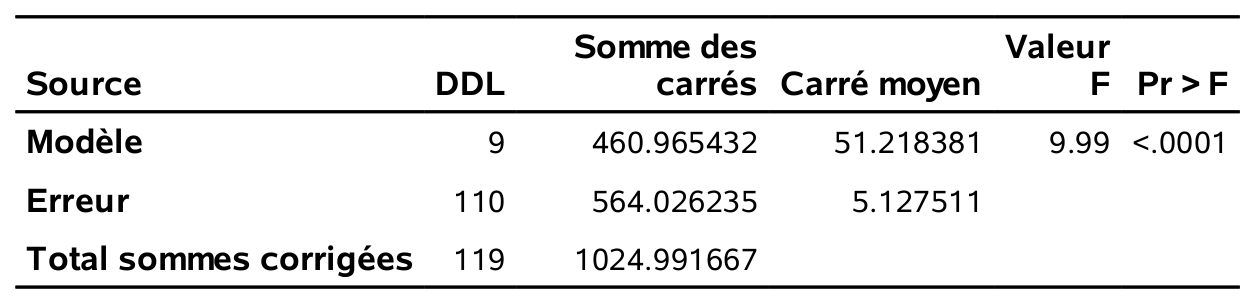
\includegraphics[width = 0.7\linewidth]{img/c2/diapos3-e12}
\end{center}
\item On rejette $\Hy_0$, ce qui veut dire que l'effet linéaire d'au moins un régresseur est non-nul pour décrire l'intention d'achat.
\ei
\end{frame}



\begin{frame}[fragile]
\frametitle{Décomposition de la somme des carrés}
 \bi \item Les comparaisons de modèles emboîtés sont effectuées avec la somme des carrés de \textbf{type III}.
 \bi \item le modèle contraint inclut toutes les variables explicatives, hormis celle testée.
 \ei \item La somme des carrés de type I fait des \textbf{comparaisons séquentielles}. Pour la $j$e covariable, on compare le modèle avec les variables préalablements ajoutées --- l'ordre d'entrée des variables explicatives devient important.
 \bi \item par exemple, si la première variable ajoutée est celle dont vous voulez tester l'effet, la comparaison est entre un modèle avec seulement cette variable et le modèle avec uniquement l'ordonnée à l'origine.
 \ei
 \item Pour éviter de vous tromper dans l'interprétation, ajoutez \code{ss3} dans votre appel \SASlang.
 \ei 
\end{frame}


\begin{frame}[fragile]
\frametitle{Test-$F$ global pour variables catégorielles}

\bi
% \item \SASlang also reports global tests for each of the variables.
\item Quand la $j$e variable explicative est continue ou binaire, le test-$F$ est  \alert{équivalent} au test-$t$ pour $\beta_j=0$. Ces variables ont \code{DDL=1}.
\item Quand les variables sont catégorielles (telles que définies par  \code{class} en \SASlang), la sortie est différente. Par exemple, le test global pour une variable catégorielle \code{cat} à $k$ niveaux correspond à l'hypothèse $\Hy_0: \beta_{\code{cat}_1}= \cdots = \beta_{\code{cat}_{k-1}}=0$
\item comparer le modèle avec ou sans cette variable catégorielle, en prenant en compte l'effet de toutes les autres variables.
\ei
\end{frame}
\begin{frame}[fragile]
Supposez qu'on ajuste un modèle linéaire avec toutes les variables explicatives des données \code{intention}.
\begin{tcolorbox}[colback=white, colframe=hecblue, title=Code \SASlang pour ajuste le modèle linéaire complet]
\begin{verbatim}
proc glm data=modstat.intention noprint;
class sexe educ revenu;
model intention= fixation emotion 
    sexe age revenu educ statut / ss3 solution;
run;
\end{verbatim}
\end{tcolorbox}
\end{frame}
\begin{frame}

\bi \item 
Les degrés de libertés pour \code{revenu} et \code{educ} sont deux, parce que chaque variable a trois catégories.
\item par exemple, le test $F$ compare le modèle avec toutes les variables explicatives à celui sans éducation, $\beta_{\code{educ}_1} = \beta_{\code{educ}_2}=0$.
\ei
\begin{center}
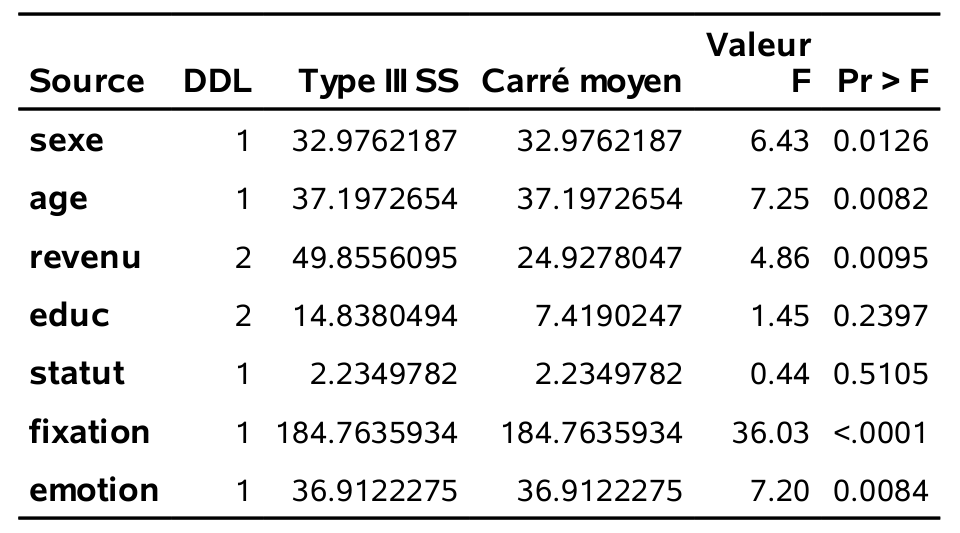
\includegraphics[width = 0.7\linewidth]{img/c2/diapos3-e10.png}
\end{center}

\end{frame}


\end{document}
